\documentclass[a4paper,11pt]{article}
\usepackage{amsmath,amsthm,amsfonts,amssymb,amscd,amstext,vmargin,graphics,graphicx,tabularx,multicol} \usepackage[french]{babel}
\usepackage[utf8]{inputenc}  
\usepackage[T1]{fontenc} 
\usepackage[T1]{fontenc}
\usepackage{amsmath,amssymb}
\usepackage{pstricks-add,tikz,tkz-tab,variations}
\usepackage[autolanguage,np]{numprint} 
\usepackage{color}
\usepackage{ulem}

\setmarginsrb{1.5cm}{0.5cm}{1cm}{0.5cm}{0cm}{0cm}{0cm}{0cm} %Gauche, haut, droite, haut
\newcounter{numexo}
\newcommand{\exo}[1]{\stepcounter{numexo}\noindent{\bf Exercice~\thenumexo} : \marginpar{\hfill /#1}}
\reversemarginpar


\newcounter{enumtabi}
\newcounter{enumtaba}
\newcommand{\q}{\stepcounter{enumtabi} \theenumtabi.  }
\newcommand{\qa}{\stepcounter{enumtaba} (\alph{enumtaba}) }
\newcommand{\initq}{\setcounter{enumtabi}{0}}
\newcommand{\initqa}{\setcounter{enumtaba}{0}}

\newcommand{\be}{\begin{enumerate}}
\newcommand{\ee}{\end{enumerate}}
\newcommand{\bi}{\begin{itemize}}
\newcommand{\ei}{\end{itemize}}
\newcommand{\bp}{\begin{pspicture*}}
\newcommand{\ep}{\end{pspicture*}}
\newcommand{\bt}{\begin{tabular}}
\newcommand{\et}{\end{tabular}}
\renewcommand{\tabularxcolumn}[1]{>{\centering}m{#1}} %(colonne m{} centrée, au lieu de p par défault) 
\newcommand{\tnl}{\tabularnewline}

\newcommand{\trait}{\noindent \rule{\linewidth}{0.2mm}}
\newcommand{\hs}[1]{\hspace{#1}}
\newcommand{\vs}[1]{\vspace{#1}}

\newcommand{\N}{\mathbb{N}}
\newcommand{\Z}{\mathbb{Z}}
\newcommand{\R}{\mathbb{R}}
\newcommand{\C}{\mathbb{C}}
\newcommand{\Dcal}{\mathcal{D}}
\newcommand{\Ccal}{\mathcal{C}}
\newcommand{\mc}{\mathcal}

\newcommand{\vect}[1]{\overrightarrow{#1}}
\newcommand{\ds}{\displaystyle}
\newcommand{\eq}{\quad \Leftrightarrow \quad}
\newcommand{\vecti}{\vec{\imath}}
\newcommand{\vectj}{\vec{\jmath}}
\newcommand{\Oij}{(O;\vec{\imath}, \vec{\jmath})}
\newcommand{\OIJ}{(O;I,J)}

\newcommand{\bmul}[1]{\begin{multicols}{#1}}
\newcommand{\emul}{\end{multicols}}


\newcommand{\reponse}[1][1]{%
\multido{}{#1}{\makebox[\linewidth]{\rule[0pt]{0pt}{20pt}\dotfill}
}}

\newcommand{\titre}[5] 
% #1: titre #2: haut gauche #3: bas gauche #4: haut droite #5: bas droite
{
\noindent #2 \hfill #4 \\
#3 \hfill #5

\vspace{-1.6cm}

\begin{center}\rule{6cm}{0.5mm}\end{center}
\vspace{0.2cm}
\begin{center}{\large{\textbf{#1}}}\end{center}
\begin{center}\rule{6cm}{0.5mm}\end{center}
}



\begin{document}
\pagestyle{empty}
\titre{ Interrogation : Les fonctions affines}{Nom}{Prénom}{Date}{Classe}





\exo{2} Les fonctions suivantes sont-elles affines ? Si oui, précisez si elles sont linéaires ou constantes et précisez leur coefficient.\\

\bmul{4}


$ h : x \longmapsto 10x^{2}+5$ 


\columnbreak

$ g : x \longmapsto \dfrac{x}{7}$ 



\columnbreak


$ f : x \longmapsto 3x-7$ 


\columnbreak

$ i : x \longmapsto \dfrac{6x-1}{5}$ 



\emul

\noindent \reponse[5]\\



\exo{2.5} \\
$f$ est une fonction affine telle que $f(1) = 12$ et $f(4) = 3$. Retrouver l'expression algébrique de cette fonction. \\
\reponse[11]\\




\exo{5.5}

Trois jeunes amis décident de travailler le soir après les cours pour gagner un peu d'argent. Comme ils ont le permis de conduire, ils s'orientent vers la livraison de pizzas. Ils ont réussi à trouver un emploi dans trois pizzerias différentes.\\
• David va recevoir un salaire fixe de 70 000 F par mois.\\
• Guillaume aura un salaire mensuel composé d'une partie fixe de 50 000 F à
laquelle s'ajoutent 100 F par livraison effectuée.\\
• Angelo sera payé chaque mois 200 F par livraison.\\

\initq \q Si durant un mois les pizzerias ne reçoivent que très peu de commandes (moins de 200), qui devrait gagner le plus d'argent ? Justifier votre réponse par des calculs.\\
\reponse[4]\\

 Dans cette question, x désigne le nombre de livraisons effectuées durant un mois. f , g et h sont trois fonctions représentant respectivement le salaire de David, Guillaume et Angelo.\\
\q Écrire l'expression algébrique de chacune de ces fonctions. Aucune justification n'est attendue.\\
\reponse[3]\\

\q Durant un mois, combien de livraisons Guillaume doit-il effectuer pour
avoir le même salaire que celui de David ?\\
\reponse[5]\\


\q \initqa  \qa Dans le repère ci-dessous, écrire le nom de la fonction correspondant
à chaque droite.\\

\qa À l'aide du graphique, déterminer le nombre de livraisons à partir duquel Angelo sera celui qui recevra le plus gros salaire mensuel.\\
\reponse[2]


\includegraphics[scale=0.75]{fonctionsaffines.eps} 

\end{document}
